\documentclass[aspectratio=169]{beamer}

\usepackage[T1,T2A]{fontenc}
\usepackage[main=russian,english]{babel}

\usepackage{cmap}
\usepackage{tikz}
\usepackage{array}
\usepackage{multicol}
\usepackage{booktabs}
\usepackage{csquotes}
\usepackage{amssymb,amsfonts,amsmath}
\usepackage{algorithm}
\usepackage{algpseudocode}
\usepackage{mdframed}

% Настройки стиля из предоставленного шаблона
\usecolortheme{beaver}
\usefonttheme[onlymath]{serif}
\setbeamertemplate{navigation symbols}{}
\setbeamertemplate{footline}[page number]
\setbeamertemplate{blocks}[rounded=true,shadow=true]
\setbeamersize{text margin left=0.5cm,text margin right=0.5cm}
\setbeamerfont{author}{size=\normalsize}
\setbeamerfont{institute}{size=\normalsize}
\setbeamerfont{date}{size=\normalsize}
\setbeamercolor{block title}{fg=white,bg=gray!70!black}
\setbeamercolor{block body}{fg=black,bg=green!5!white}
\setbeamertemplate{enumerate item}{\insertenumlabel)}
\setbeamertemplate{enumerate subitem}{\insertenumlabel)}
\setbeamertemplate{enumerate subsubitem}{\insertenumlabel)}
\newmdenv[
    nobreak=true,
    skipabove=\topskip,
    skipbelow=\topskip,
    linewidth=1pt
]{nframed}

% Метаданные доклада
\title{Алгоритм типа UCB для обучения экспертов при ограниченном бюджете}
\author{
    Латыпов~Ильгам~Магданович\\
    \vspace{0.2cm}
    {\small Научный руководитель: кандидат технических наук Дорн~Ю.~В.}
}
\institute{
    Кафедра интеллектуальных систем ФПМИ МФТИ\\
    Специализация: Интеллектуальный анализ данных\\
    Направление: Информатика и вычислительная техника
}
\date{\today}

\begin{document}

\begin{frame}
  \titlepage
\end{frame}

\begin{frame}{План работы}
\small
Исследуется задача последовательного принятия решений с обучаемыми экспертами с учетом вычислительных бюджетов.

\textbf{Проблема:} Существующие подходы выбора экспертов для последовательного принятия решений либо не учитывают динамику обучения экспертов, из-за чего слишком мало исследуют медленно обучаемых экспертов, либо не учитывают наличие дополнительных вычислительных ресурсов на раундах и обучаются медленнее чем могли бы.

\vspace{0.25cm}
\textbf{Задача:} Предложить алгоритм выбора экспертов, который учитывает обе модальности: динамику обучения и ограничения на вычислительный бюджет и провести теоретический анализ качества его работы.
\end{frame}

\begin{frame}{Эксперты, потери и протокол}
\small
\begin{block}{Среда и функция потерь}
Пространство решений: $\mathbf{U}$, пространство исходов: $\mathbf{E}$.

Функция потерь: $\ell:\mathbf{U}\times\mathbf{E}\to\mathbb{R}_+$.
\end{block}

\begin{block}{Эксперт}
Эксперт $k\in[K]$ работает на подпространстве $\mathbf{U}_k\subseteq\mathbf{U}$ и на раунде $t$ выдает решение $u_k^t\in\mathbf{U}_k$.
\end{block}

\begin{nframed}
\textbf{Протокол}
\begin{enumerate}
    \item выбрать $S_t\subseteq[K]$, $|S_t|\le M$, и решение $u^t\in\mathbf{U}$;
    \item наблюдать $\xi^t\sim D$ и понести потери $\ell(u^t,\xi^t)$;
    \item для каждого $k\in S_t$ вычислить $\ell(u_k^t,\xi^t)$ и обновить эксперта $k$.
\end{enumerate}
\end{nframed}
\end{frame}

\begin{frame}{Постановка цели процедуры}
\small

\textbf{Ожидаемые потери решения:}
\[
L(u):=\mathbb{E}_{\xi\sim\mathcal{D}}[\ell(u,\xi)],\quad
L_k^\star:=\min_{u\in\mathbf{U}_k}L(u),\quad
L^\star:=\min_{k\in[K]}L_k^\star.
\]

\textbf{Сожаление процедуры:}
\[
\mathrm{Reg}(T):=\sum_{t=1}^T\ell(u^t,\xi^t)-T\cdot L^\star.
\]

\begin{block}{Предположение: Стохастическая среда}
\[
\xi^t\overset{\mathrm{iid}}{\sim}D,\qquad \ell:\mathbf{U}\times\mathbf{E}\to[0,1].
\]
\end{block}
\end{frame}

\begin{frame}{Эксперты: предположение и обозначения}
\small
\textbf{История обучения и потери:}
\begin{align}
I_k(t):=\{\tau<t:\;k\in S_\tau\},\qquad n_k^t:=|I_k(t)|, \\
L_k(t):=\frac{1}{n_k^t}\sum_{\tau\in I_k(t)}\ell(u_k^\tau,\xi^\tau)
\end{align}

\textbf{Внутреннее сожаление эксперта:}
\[
R_k(t):=n_k^t\big(L_k(t)-L_k^\star\big).
\]

\begin{block}{Предположение: Равномерное по времени ограничение сожаления эксперта}
Для эксперта $k$ для любого $\delta\in(0,1)$, с вероятностью не менее $1-\delta$, для всех $t\ge1$,
\[
R_k(t)\le U_k(n_k^t,\delta),
\]
% где $U_k(\cdot,\delta)$ неубывает.
\end{block}

\textbf{Идея: Введем доверительные границы на оптимальную потерю эксперта}
\[
\mathrm{LCB}(k,n_k^t,\delta),\;\mathrm{UCB}(k,n_k^t,\delta).
\]
\end{frame}

\begin{frame}{Доверительный интервал эксперта: структура и лемма}
\small
\[
\mathrm{LCB}(k,n_k^t,\delta)=L_k(t)-\underbrace{\frac{U_k(n_k^t,\frac{\delta}{2K})}{n_k^t}}_{\text{скорость обучения}}-\underbrace{c_1\sqrt{\frac{\log(4K(n_k^t)^2/\delta)}{n_k^t}}}_{\text{слагаемое концентрации}},
\]
\[
\mathrm{UCB}(k,n_k^t,\delta)=L_k(t)+\underbrace{c_2\sqrt{\frac{\log(4K(n_k^t)^2/\delta)}{n_k^t}}}_{\text{слагаемое концентрации}}.
\]

\begin{lemma}[Корректность доверительных интервалов (Латыпов, 2026)]
С вероятностью не менее $1-\delta$ для любого $k$ и любого $t\ge1$ выполняется
\[
\mathrm{LCB}(k,n_k^t,\delta)\le L_k^\star\le\mathrm{UCB}(k,n_k^t,\delta).
\]
\end{lemma}
\end{frame}

\begin{frame}{Алгоритм M-LCB}
\footnotesize
\begin{algorithmic}[1]
\State \textbf{Input:} эксперты $\{\mathbf{U}_k\}_{k=1}^K$, бюджет $M$, параметр уверенности $\delta$, smoothing wrapper $\upsilon$
\State \textbf{Output:} советы $\{u^t\}_{t=1}^T$, обучаемые множества $\{S_t\}_{t=1}^T$
\State Инициализировать $\delta_{\mathrm{arm}}\gets\delta/(2K)$ и сделать warm-start каждого эксперта
\For{$t=1,2,\dots,T$}
    \For{$k\in[K]$}
        \State Вычислить $\mathrm{LCB}_k(t,\delta),\mathrm{UCB}_k(t,\delta)$
    \EndFor
    \State $S_t\gets\arg\min_{S\subseteq[K],|S|=M}\sum_{k\in S}\mathrm{LCB}_k(t,\delta)$
    \State $i_t\gets\arg\min_{k\in S_t}\mathrm{UCB}_k(t,\delta)$
    \State $u^t\gets\upsilon(\{u_{i_t}^{\tau}:\tau\in I_{i_t}(t)\})$ \Comment{сглаживание эксперта $i_t$}
    \State Сыграть $u^t$, получить $\ell(u^t,\xi^t)$
    \For{$k\in S_t$}
        \State Наблюдать $\ell(u_k^t,\xi^t)$ и обновить эксперта $k$
    \EndFor
\EndFor
\end{algorithmic}
\end{frame}

\begin{frame}{Гарантии на глобальное сожаление}
\footnotesize
Для ранее введенного сожаления
$\mathrm{Reg}(T):=\sum_{t=1}^T\ell(u^t,\xi^t)-T\cdot L^\star$
получены следующие оценки.

\begin{lemma}[Оценка сожаления (Латыпов, 2026)]
С вероятностью не менее $1-\delta$,
\begin{align*}
\mathrm{Reg}(T) \le&
\sum_{\tau \in I_{k^\star}(T)}
\bigl[\mathrm{UCB}_{k^\star}(\tau,\delta)-\mathrm{LCB}_{k^\star}(\tau,\delta)\bigr]
+ \frac{1}{M}\sum_{k=1}^K \sum_{\tau \in I_k(T)}
\bigl[\mathrm{UCB}_k(\tau,\delta)-\mathrm{LCB}_k(\tau,\delta)\bigr].
\end{align*}
\end{lemma}

\begin{theorem}[Convergence rates (Латыпов, 2026)]
Пусть $\alpha,\delta\in(0,1)$, и каждый эксперт $k$ удовлетворяет предположению о внутреннем сожалении
\[
U_k(t,\delta)=O\big(t^\alpha c(\delta)\big).
\]
Тогда с вероятностью не менее $1-\delta$ сожаление алгоритма M-LCB ограничено для всех $T\ge1$:
\[
\mathrm{Reg}(T)=O\!\left(\sqrt{\frac{KT}{M}\log\!\frac{KT}{\delta}}+\Bigl(\frac{K}{M}\Bigr)^{1-\alpha}T^{\alpha}c(\delta)\right).
\]
\end{theorem}
\end{frame}

\begin{frame}{Гарантия на усредненное сожаление Top-$M$}
\small
\textbf{Среднее сожаление выбранного множества:}
\[
\mathrm{Reg}_M(T):=\sum_{t=1}^T\left[\frac{1}{M}\sum_{k\in S_t}L_k^\star-\overline{L}^\star\right],
\quad
\overline{L}^\star=\min_{|S|=M}\frac{1}{M}\sum_{k\in S}L_k^\star.
\]

\begin{theorem}[Top-$M$ mean regret / усредненное сожаление (Латыпов, 2026)]
Пусть $\alpha,\delta\in(0,1)$, и каждый эксперт $k$ удовлетворяет предположению о внутреннем сожалении
\[
U_k(t,\delta)=O\big(t^\alpha c(\delta)\big).
\]
Тогда с вероятностью не менее $1-\delta$ усредненное сожаление алгоритма M-LCB ограничено для всех $T\ge1$:
\[
\mathrm{Reg}_M(T)=O\!\left(\sqrt{\frac{KT}{M}\log\!\frac{KT}{\delta}}+\Bigl(\frac{K}{M}\Bigr)^{1-\alpha}T^{\alpha}c(\delta)\right).
\]
\end{theorem}

Гарантия означает, что алгоритм системно дообучает \textbf{top-$M$ лучших} экспертов,
поэтому устойчив к неопределенности внутри этого множества.
\end{frame}

\begin{frame}{Lower bounds: фундаментальная цена задачи}
\small
\begin{theorem}[Lower bound (Латыпов, 2026)]
Для класса задач $\mathcal{F}_\alpha$,
\[
\sup_{f_k\in\mathcal{F}_{\alpha},\,k\in[K]}\mathbb{E}\,\mathrm{Reg}(T)
\ge c_1\sqrt{\frac{KT}{M}} + c_2T^\alpha\left(\frac{K}{M}\right)^{1-\alpha}.
\]
\end{theorem}

Следствие:
\begin{enumerate}
    \item при $\alpha<1/2$ доминирует цена exploration $\sqrt{KT/M}$;
    \item при $\alpha\ge1/2$ доминирует цена дообучения $T^\alpha(K/M)^{1-\alpha}$.
\end{enumerate}

Для ограниченных потерь M-LCB совпадает с нижней границей по порядку с точностью до логарифмов.
\end{frame}

\begin{frame}{Эксперимент: дизайн и проверяемая гипотеза}
\small
Сценарий: $K=10$ гетерогенных экспертов ($\varepsilon$-Greedy и UCB1), бюджеты $M\in\{1,2,3,4\}$.
\begin{enumerate}
    \item Ловушка: слабые эксперты сходятся быстрее и доминируют в начале.
    \item Гипотеза: M-LCB перераспределяет бюджет так, чтобы найти истинно сильного эксперта.
    \item Бейзлайны: LimitedAdvice и Smooth Corral.
\end{enumerate}
Метрики: накопленное сожаление, частота выбора экспертов, доля шагов обучения.
\end{frame}

\begin{frame}{Эксперимент: результаты согласуются с теорией}
\centering
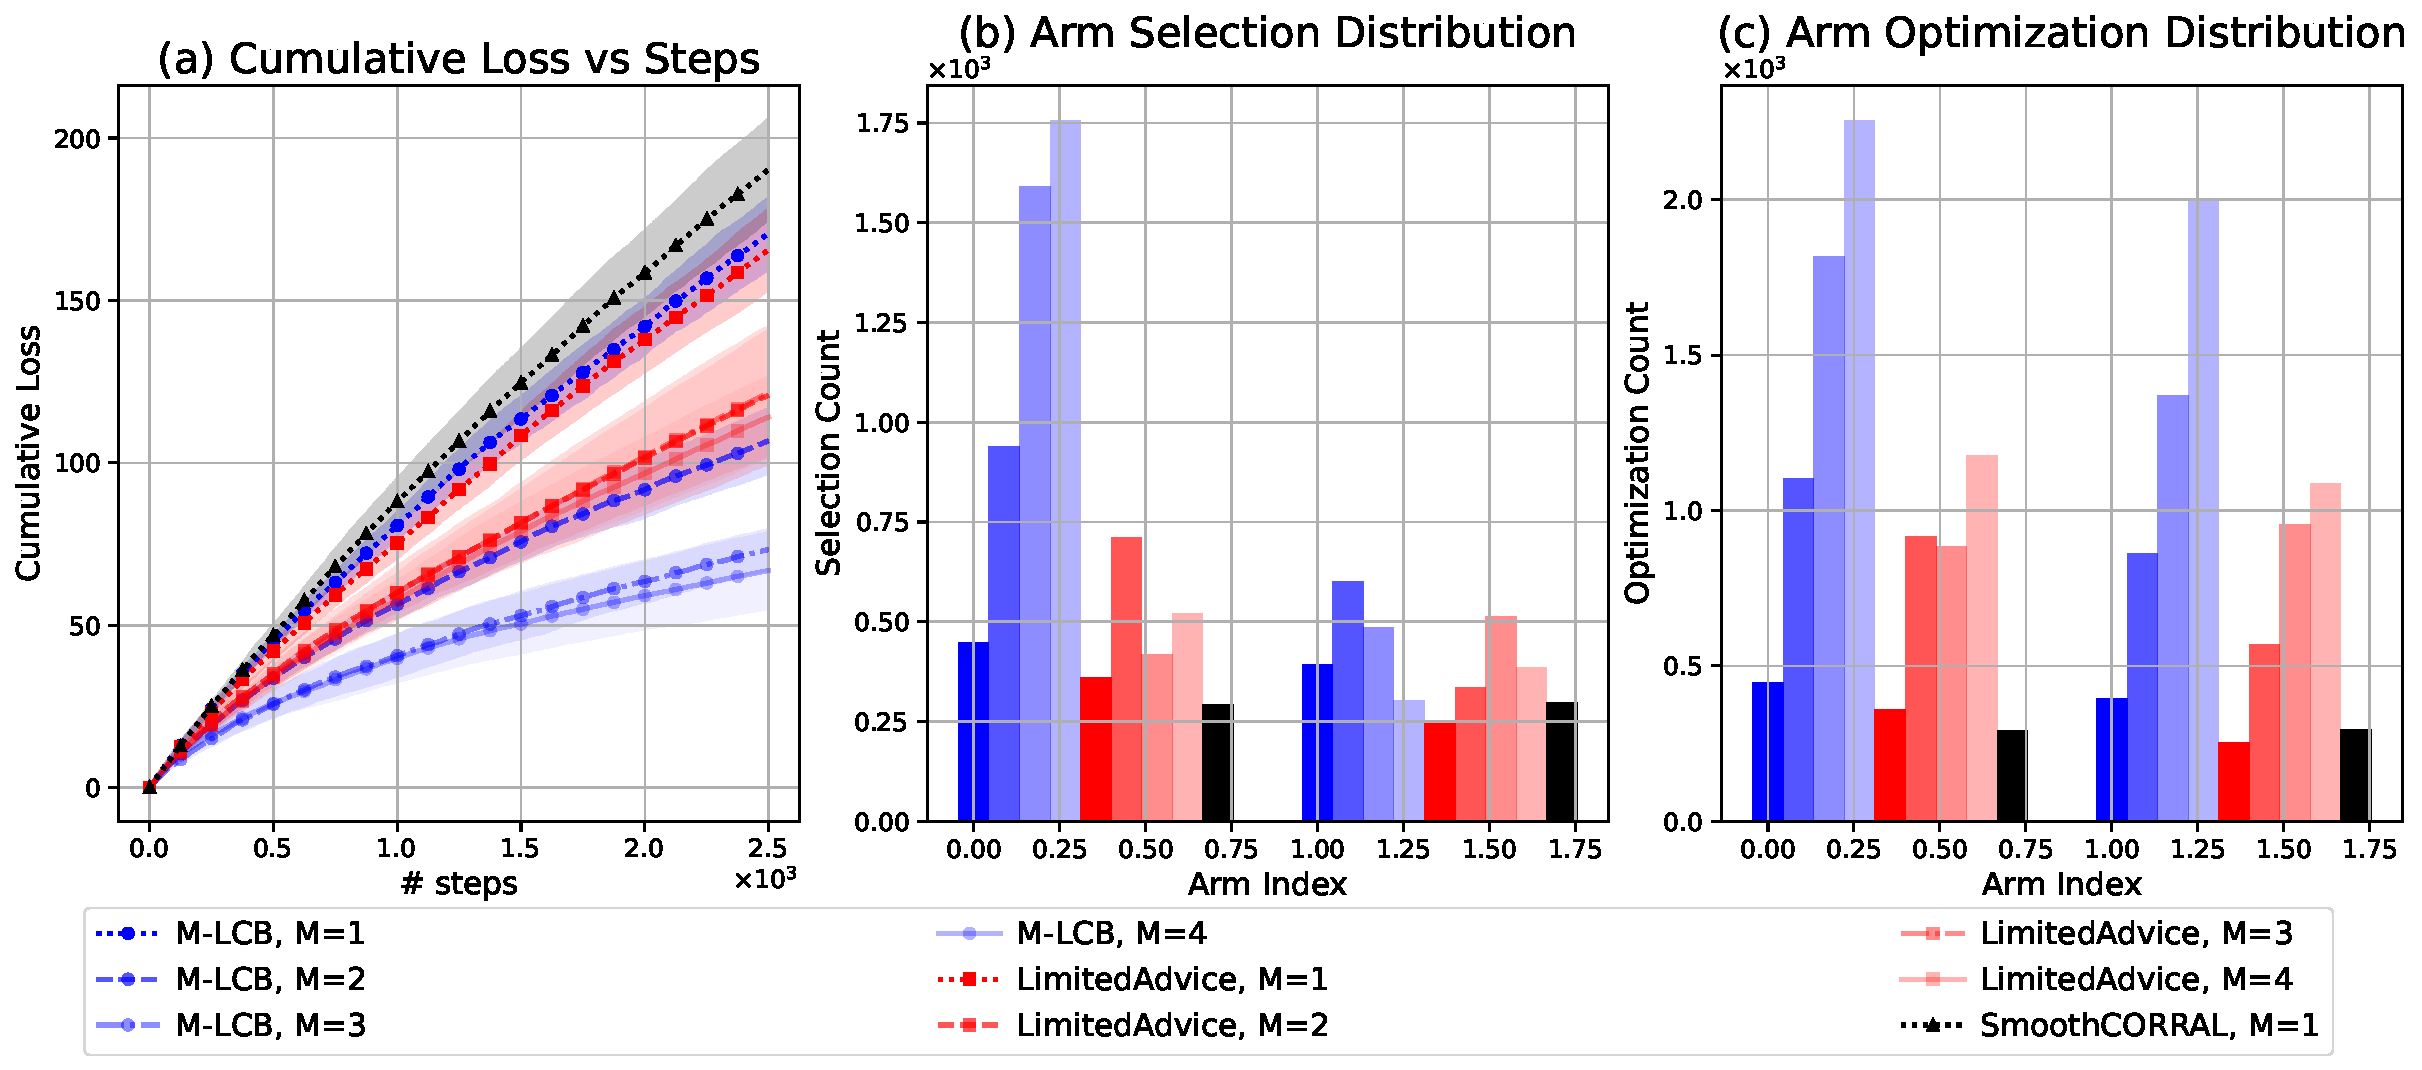
\includegraphics[height=0.58\textheight,keepaspectratio]{figures/regenerated_bandit_summary.pdf}

\vspace{0.2cm}
\raggedright
\footnotesize
Итог 1: у M-LCB более медленный рост сожаления при всех проверенных бюджетах $M$.

Итог 2: M-LCB быстрее уходит от субоптимальной ловушки и перераспределяет обучение к сильным экспертам.

Итог 3: наблюдаемая динамика согласуется с \textbf{теоремой Convergence rates} и \textbf{теоремой о Top-$M$ усредненном сожалении}.
\end{frame}

\begin{frame}{Выносится на защиту}
\small
\begin{enumerate}
    \item \textbf{Основной результат:} алгоритм M-LCB для оркестрации обучаемых экспертов при бюджете $M$ с теоретической гарантией на $\mathrm{Reg}(T)$.
    \item \textbf{Доверительные интервалы эксперта} (LCB/UCB) и лемма об их корректности при учете внутренней обучаемости экспертов.
    \item \textbf{Гарантия на усредненное сожаление Top-$M$:} обучение устойчиво выделяет и поддерживает множество лучших экспертов.
    \item \textbf{Нижняя граница задачи:} доказана фундаментальная цена $\sqrt{KT/M}+T^\alpha(K/M)^{1-\alpha}$ и показана порядковая оптимальность M-LCB.
\end{enumerate}

\vspace{0.2cm}
\small Публикации по теме: Латыпов И. М., Дорн Ю. В. \enquote{Learnable Experts Orchestration With Multi-Armed Bandits}, submitted, 2026.
\end{frame}

\end{document}
